\documentclass[11pt]{standalone}
\usepackage{tikz}
\usepackage{amssymb}
\begin{document}
% GEOMIRA export: TikZ. One unit is 18.942261bp (25.256349 px on screen).
% Needs \usepackage{tikz} and \usepackage{amssymb}.
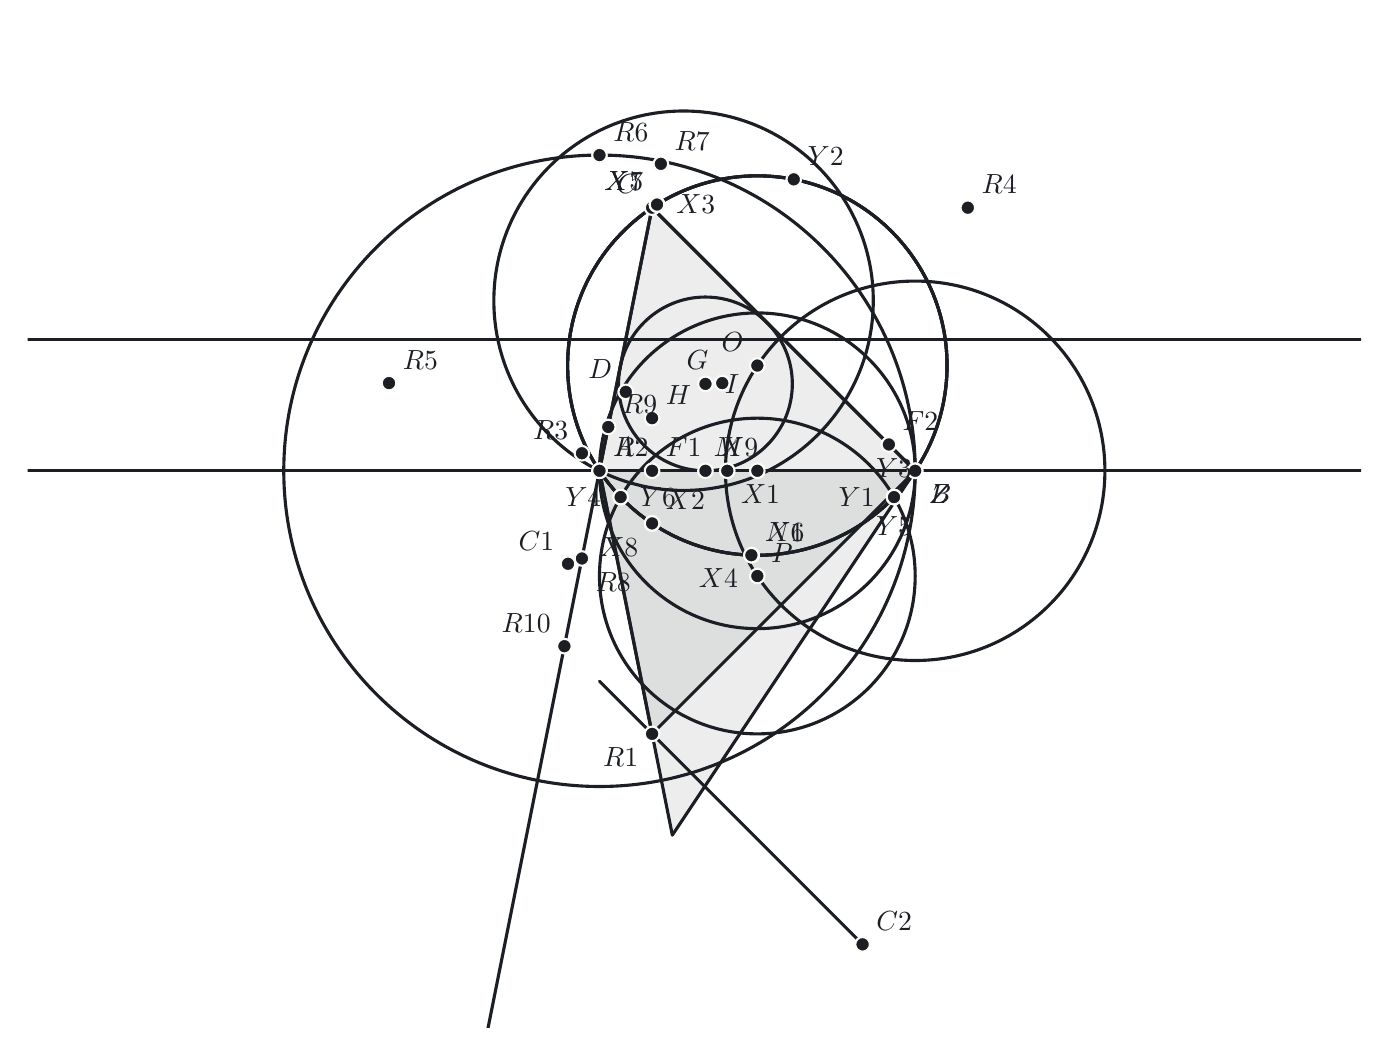
\begin{tikzpicture}[x=18.942261bp, y=18.942261bp, line cap=round, line join=round]
\definecolor{gmc0}{HTML}{1B1F24}
\definecolor{gmc1}{HTML}{FBFBF8}
\clip (-10.8673,-10.5838) rectangle (14.4729,8.4214);
% t
\fill[gmc0, fill opacity=0.08] (0,0) -- (6,0) -- (1,5) -- cycle;
\draw[gmc0, line width=1.125bp] (0,0) -- (6,0);
\draw[gmc0, line width=1.125bp] (6,0) -- (1,5);
\draw[gmc0, line width=1.125bp] (1,5) -- (0,0);
% t1
\fill[gmc0, fill opacity=0.08] (0,0) -- (1.3846,-6.9231) -- (6,0) -- cycle;
\draw[gmc0, line width=1.125bp] (0,0) -- (1.3846,-6.9231);
\draw[gmc0, line width=1.125bp] (1.3846,-6.9231) -- (6,0);
\draw[gmc0, line width=1.125bp] (6,0) -- (0,0);
% t2
\fill[gmc0, fill opacity=0.08] (0,0) -- (6,0) -- (1,-5) -- cycle;
\draw[gmc0, line width=1.125bp] (0,0) -- (6,0);
\draw[gmc0, line width=1.125bp] (6,0) -- (1,-5);
\draw[gmc0, line width=1.125bp] (1,-5) -- (0,0);
% w
\draw[gmc0, line width=1.125bp] (6.6056,2) arc[start angle=0, end angle=360, radius=3.60555];
% i
\draw[gmc0, line width=1.125bp] (3.665,1.6511) arc[start angle=0, end angle=360, radius=1.65107];
% c1
\draw[gmc0, line width=1.125bp] (6.6056,2) arc[start angle=0, end angle=360, radius=3.60555];
% c2
\draw[gmc0, line width=1.125bp] (6,-2) arc[start angle=0, end angle=360, radius=3];
% c3
\draw[gmc0, line width=1.125bp] (6.6056,2) arc[start angle=0, end angle=360, radius=3.60555];
% k1
\draw[gmc0, line width=1.125bp] (6,0) arc[start angle=0, end angle=360, radius=6];
% k2
\draw[gmc0, line width=1.125bp] (6,0) arc[start angle=0, end angle=360, radius=3];
% w1
\draw[gmc0, line width=1.125bp] (9.6056,0) arc[start angle=0, end angle=360, radius=3.60555];
% w2
\draw[gmc0, line width=1.125bp] (5.2036,3.2321) arc[start angle=0, end angle=360, radius=3.60555];
% l
\draw[gmc0, line width=1.125bp] (-13.5597,0) -- (17.1652,0);
% s1
\draw[gmc0, line width=1.125bp] (6,0) -- (1,5);
% r1
\draw[gmc0, line width=1.125bp] (1,5) -- (-2.6552,-13.2762);
% l1
\draw[gmc0, line width=1.125bp] (17.1652,2.5) -- (-13.5597,2.5);
% s2
\draw[gmc0, line width=1.125bp] (0,-4) -- (5,-9);
% A
\filldraw[fill=gmc0, draw=gmc1, line width=0.75bp] (0,0) circle[radius=2.625bp];
% B
\filldraw[fill=gmc0, draw=gmc1, line width=0.75bp] (6,0) circle[radius=2.625bp];
% C
\filldraw[fill=gmc0, draw=gmc1, line width=0.75bp] (1,5) circle[radius=2.625bp];
% P
\filldraw[fill=gmc0, draw=gmc1, line width=0.75bp] (3,-2) circle[radius=2.625bp];
% M
\filldraw[fill=gmc0, draw=gmc1, line width=0.75bp] (3,0) circle[radius=2.625bp];
% F1
\filldraw[fill=gmc0, draw=gmc1, line width=0.75bp] (1,0) circle[radius=2.625bp];
% F2
\filldraw[fill=gmc0, draw=gmc1, line width=0.75bp] (5.5,0.5) circle[radius=2.625bp];
% O
\filldraw[fill=gmc0, draw=gmc1, line width=0.75bp] (3,2) circle[radius=2.625bp];
% G
\filldraw[fill=gmc0, draw=gmc1, line width=0.75bp] (2.3333,1.6667) circle[radius=2.625bp];
% H
\filldraw[fill=gmc0, draw=gmc1, line width=0.75bp] (1,1) circle[radius=2.625bp];
% I
\filldraw[fill=gmc0, draw=gmc1, line width=0.75bp] (2.014,1.6511) circle[radius=2.625bp];
% X1
\filldraw[fill=gmc0, draw=gmc1, line width=0.75bp] (2.4286,0) circle[radius=2.625bp];
% X2
\filldraw[fill=gmc0, draw=gmc1, line width=0.75bp] (1,-1) circle[radius=2.625bp];
% X3
\filldraw[fill=gmc0, draw=gmc1, line width=0.75bp] (1.0933,5.0601) circle[radius=2.625bp];
% X4
\filldraw[fill=gmc0, draw=gmc1, line width=0.75bp] (2.893,-1.604) circle[radius=2.625bp];
% X5
\filldraw[fill=gmc0, draw=gmc1, line width=0.75bp] (1.0933,5.0601) circle[radius=2.625bp];
% X6
\filldraw[fill=gmc0, draw=gmc1, line width=0.75bp] (2.893,-1.604) circle[radius=2.625bp];
% X7
\filldraw[fill=gmc0, draw=gmc1, line width=0.75bp] (1.0933,5.0601) circle[radius=2.625bp];
% X8
\filldraw[fill=gmc0, draw=gmc1, line width=0.75bp] (1,-1) circle[radius=2.625bp];
% X9
\filldraw[fill=gmc0, draw=gmc1, line width=0.75bp] (2.014,0) circle[radius=2.625bp];
% Y1
\filldraw[fill=gmc0, draw=gmc1, line width=0.75bp] (5.5981,-0.5) circle[radius=2.625bp];
% Y2
\filldraw[fill=gmc0, draw=gmc1, line width=0.75bp] (3.6923,5.5385) circle[radius=2.625bp];
% Y3
\filldraw[fill=gmc0, draw=gmc1, line width=0.75bp] (5.5981,-0.5) circle[radius=2.625bp];
% Y4
\filldraw[fill=gmc0, draw=gmc1, line width=0.75bp] (0.4019,-0.5) circle[radius=2.625bp];
% Y5
\filldraw[fill=gmc0, draw=gmc1, line width=0.75bp] (5.5981,-0.5) circle[radius=2.625bp];
% Y6
\filldraw[fill=gmc0, draw=gmc1, line width=0.75bp] (0.4019,-0.5) circle[radius=2.625bp];
% Z
\filldraw[fill=gmc0, draw=gmc1, line width=0.75bp] (6,0) circle[radius=2.625bp];
% N1
\filldraw[fill=gmc0, draw=gmc1, line width=0.75bp] (2.8868,-1.6038) circle[radius=2.625bp];
% C1
\filldraw[fill=gmc0, draw=gmc1, line width=0.75bp] (-0.5981,-1.7679) circle[radius=2.625bp];
% C2
\filldraw[fill=gmc0, draw=gmc1, line width=0.75bp] (5,-9) circle[radius=2.625bp];
% R1
\filldraw[fill=gmc0, draw=gmc1, line width=0.75bp] (1,-5) circle[radius=2.625bp];
% R2
\filldraw[fill=gmc0, draw=gmc1, line width=0.75bp] (0,0) circle[radius=2.625bp];
% R3
\filldraw[fill=gmc0, draw=gmc1, line width=0.75bp] (-0.3333,0.3333) circle[radius=2.625bp];
% R4
\filldraw[fill=gmc0, draw=gmc1, line width=0.75bp] (7,5) circle[radius=2.625bp];
% R5
\filldraw[fill=gmc0, draw=gmc1, line width=0.75bp] (-4,1.6667) circle[radius=2.625bp];
% R6
\filldraw[fill=gmc0, draw=gmc1, line width=0.75bp] (0,6) circle[radius=2.625bp];
% R7
\filldraw[fill=gmc0, draw=gmc1, line width=0.75bp] (1.1667,5.8333) circle[radius=2.625bp];
% R8
\filldraw[fill=gmc0, draw=gmc1, line width=0.75bp] (-0.3333,-1.6667) circle[radius=2.625bp];
% R9
\filldraw[fill=gmc0, draw=gmc1, line width=0.75bp] (0.1667,0.8333) circle[radius=2.625bp];
% R10
\filldraw[fill=gmc0, draw=gmc1, line width=0.75bp] (-0.6667,-3.3333) circle[radius=2.625bp];
% D
\filldraw[fill=gmc0, draw=gmc1, line width=0.75bp] (0.5,1.5) circle[radius=2.625bp];
\node[anchor=south west, inner sep=0pt, text=gmc0] at (0.252,0.252) {$A$}; % label of A
\node[anchor=north west, inner sep=0pt, text=gmc0] at (6.252,-0.252) {$B$}; % label of B
\node[anchor=south east, inner sep=0pt, text=gmc0] at (0.748,5.252) {$C$}; % label of C
\node[anchor=south west, inner sep=0pt, text=gmc0] at (3.252,-1.748) {$P$}; % label of P
\node[anchor=south east, inner sep=0pt, text=gmc0] at (2.748,0.252) {$M$}; % label of M
\node[anchor=south west, inner sep=0pt, text=gmc0] at (1.252,0.252) {$F1$}; % label of F1
\node[anchor=south west, inner sep=0pt, text=gmc0] at (5.752,0.752) {$F2$}; % label of F2
\node[anchor=south east, inner sep=0pt, text=gmc0] at (2.748,2.252) {$O$}; % label of O
\node[anchor=south east, inner sep=0pt, text=gmc0] at (2.0814,1.9186) {$G$}; % label of G
\node[anchor=south west, inner sep=0pt, text=gmc0] at (1.252,1.252) {$H$}; % label of H
\node[anchor=west, inner sep=0pt, text=gmc0] at (2.3703,1.6511) {$I$}; % label of I
\node[anchor=north west, inner sep=0pt, text=gmc0] at (2.6805,-0.252) {$X1$}; % label of X1
\node[anchor=south west, inner sep=0pt, text=gmc0] at (1.252,-0.748) {$X2$}; % label of X2
\node[anchor=west, inner sep=0pt, text=gmc0] at (1.4496,5.0601) {$X3$}; % label of X3
\node[anchor=north east, inner sep=0pt, text=gmc0] at (2.6411,-1.8559) {$X4$}; % label of X4
\node[anchor=south east, inner sep=0pt, text=gmc0] at (0.8413,5.3121) {$X5$}; % label of X5
\node[anchor=south west, inner sep=0pt, text=gmc0] at (3.145,-1.352) {$X6$}; % label of X6
\node[anchor=south east, inner sep=0pt, text=gmc0] at (0.8413,5.3121) {$X7$}; % label of X7
\node[anchor=north east, inner sep=0pt, text=gmc0] at (0.748,-1.252) {$X8$}; % label of X8
\node[anchor=south west, inner sep=0pt, text=gmc0] at (2.266,0.252) {$X9$}; % label of X9
\node[anchor=east, inner sep=0pt, text=gmc0] at (5.2417,-0.5) {$Y1$}; % label of Y1
\node[anchor=south west, inner sep=0pt, text=gmc0] at (3.9443,5.7904) {$Y2$}; % label of Y2
\node[anchor=south, inner sep=0pt, text=gmc0] at (5.5981,-0.1437) {$Y3$}; % label of Y3
\node[anchor=east, inner sep=0pt, text=gmc0] at (0.0456,-0.5) {$Y4$}; % label of Y4
\node[anchor=north, inner sep=0pt, text=gmc0] at (5.5981,-0.8563) {$Y5$}; % label of Y5
\node[anchor=west, inner sep=0pt, text=gmc0] at (0.7583,-0.5) {$Y6$}; % label of Y6
\node[anchor=north west, inner sep=0pt, text=gmc0] at (6.252,-0.252) {$Z$}; % label of Z
\node[anchor=south west, inner sep=0pt, text=gmc0] at (3.1388,-1.3518) {$N1$}; % label of N1
\node[anchor=south east, inner sep=0pt, text=gmc0] at (-0.8501,-1.516) {$C1$}; % label of C1
\node[anchor=south west, inner sep=0pt, text=gmc0] at (5.252,-8.748) {$C2$}; % label of C2
\node[anchor=north east, inner sep=0pt, text=gmc0] at (0.748,-5.252) {$R1$}; % label of R1
\node[anchor=south west, inner sep=0pt, text=gmc0] at (0.252,0.252) {$R2$}; % label of R2
\node[anchor=south east, inner sep=0pt, text=gmc0] at (-0.5853,0.5853) {$R3$}; % label of R3
\node[anchor=south west, inner sep=0pt, text=gmc0] at (7.252,5.252) {$R4$}; % label of R4
\node[anchor=south west, inner sep=0pt, text=gmc0] at (-3.748,1.9186) {$R5$}; % label of R5
\node[anchor=south west, inner sep=0pt, text=gmc0] at (0.252,6.252) {$R6$}; % label of R6
\node[anchor=south west, inner sep=0pt, text=gmc0] at (1.4186,6.0853) {$R7$}; % label of R7
\node[anchor=north west, inner sep=0pt, text=gmc0] at (-0.0814,-1.9186) {$R8$}; % label of R8
\node[anchor=south west, inner sep=0pt, text=gmc0] at (0.4186,1.0853) {$R9$}; % label of R9
\node[anchor=south east, inner sep=0pt, text=gmc0] at (-0.9186,-3.0814) {$R10$}; % label of R10
\node[anchor=south east, inner sep=0pt, text=gmc0] at (0.248,1.752) {$D$}; % label of D
\end{tikzpicture}
\end{document}
